\documentclass[aspectratio=169]{beamer}
\usepackage{amsmath}
\usepackage{amssymb}
\usepackage{tikz}
\usepackage{xcolor}
\usetikzlibrary{shapes,backgrounds,patterns}

\usepackage{pgfplots}
\pgfplotsset{compat=1.18, legend cell align=left}
\usetikzlibrary{arrows.meta,decorations.pathreplacing,calc,positioning}
\usepackage{booktabs}
\usepackage{pifont}
\usepgfplotslibrary{fillbetween}

% royalblue isn't a base xcolor name, so define it first (this is the default accent)
\definecolor{royalblue}{RGB}{65,105,225}

% ============================================================
%  ACCENT COLOR: change ONE line below to switch the theme
%  Choose one of: royalblue , red , black
% ============================================================
\colorlet{accent}{royalblue}
% \colorlet{accent}{red}
% \colorlet{accent}{black}
% ============================================================

% colorblind-safe, high-contrast second color (Okabe-Ito vermillion)
\definecolor{hl}{RGB}{213,94,0}

\usetheme{default}
\setbeamercolor{background canvas}{bg=white}
\setbeamercolor{normal text}{fg=black}
\setbeamercolor{structure}{fg=accent}
\setbeamercolor{frametitle}{fg=accent,bg=white}
\setbeamercolor{title}{fg=accent}
\setbeamercolor{section in toc}{fg=black}
\setbeamercolor{block title}{fg=black,bg=gray!10}
\setbeamercolor{block body}{fg=black,bg=gray!5}
\setbeamercolor{block title example}{fg=black,bg=green!10}
\setbeamercolor{block body example}{fg=black,bg=green!5}
\setbeamercolor{block title alerted}{fg=black,bg=red!10}
\setbeamercolor{block body alerted}{fg=black,bg=red!5}

\setbeamertemplate{navigation symbols}{}
\setbeamertemplate{footline}{
    \hfill\makebox[5pt]{%
        \scriptsize\insertframenumber}
    \hspace*{2em}
    \vspace{0.5cm}
}

\newcommand{\cbox}[2]{\colorbox{#1}{\ensuremath{\displaystyle #2}}}

\pgfplotsset{
  miniplot/.style={
    width=4.0cm, height=3.0cm,
    axis lines=middle, xtick=\empty, ytick=\empty,
    samples=120, thick, clip=true
  }
}

\definecolor{gr}{RGB}{0,158,115}


% curve and helpers for the three-rule picture
\pgfmathdeclarefunction{fc}{1}{\pgfmathparse{0.55+1.25*sin(deg(0.85*#1))}}
\pgfmathdeclarefunction{gc}{1}{\pgfmathparse{0.55+0.3*sin(deg(#1))+1.1*exp(-4*(#1-2.6)^2)}}
\pgfplotsset{
  rule2/.style={
    width=5.4cm, height=3.6cm, axis lines=middle, xmin=0, xmax=4.3, ymin=0, ymax=1.95,
    xtick=\empty, ytick=\empty, thick, clip=false,
    title style={font=\small}
  }
}
\pgfplotsset{
  rule/.style={
    width=5.4cm, height=4.2cm, axis lines=middle, xmin=0, xmax=4.3, ymin=0, ymax=1.95,
    xtick=\empty, ytick=\empty, thick, clip=false, samples=100,
    title style={font=\small}
  }
}

\pgfplotsset{
  rev/.style={
    width=4.9cm, height=3.1cm, axis lines=middle, xmin=0, xmax=4.3, ymin=0, ymax=1.95,
    xtick=\empty, ytick=\empty, thick, clip=false,
    title style={font=\small, yshift=-4pt, text depth=0pt, text height=1.6ex}
  }
}

\title{Double Integrals and Monte Carlo Integration}
\subtitle{Integration in two dimensions with SymPy, SciPy and random sampling}
\author{Sharareh Sayyad}
\institute{Washington State University}
\date{\today}

\begin{document}
\frame{\titlepage}

% ------------------------------------------------------------
\begin{frame}{Review: integration in one dimension}
\begin{block}{Exact: SymPy}
\small
\texttt{sp.integrate(f, (x, a, b))} \quad
\footnotesize
\textcolor{gr}{\ding{51}} exact \quad
\textcolor{hl}{\ding{55}} may return \texttt{Integral(...)} $\to$ \texttt{.evalf()}
\end{block}

\vspace{0.3em}
{\usebeamercolor[fg]{structure}\textbf{Numerical: SciPy}} \ \small fit a simple shape on each piece and integrate it exactly

\vspace{0.1em}
\centering
\begin{tikzpicture}
\begin{axis}[rev, title={Trapezoid}, name=T2]
\addplot[draw=gr, very thick, fill=gr!15] coordinates {(0.4000,0.6668) (0.9667,0.7969) (1.5333,0.8614) (2.1000,1.2136) (2.6667,1.7678) (3.2333,0.7436) (3.8000,0.3699)} \closedcycle;
\draw[thin, gr!70!black] (axis cs:0.9667,0) -- (axis cs:0.9667,0.7969);
\draw[thin, gr!70!black] (axis cs:1.5333,0) -- (axis cs:1.5333,0.8614);
\draw[thin, gr!70!black] (axis cs:2.1000,0) -- (axis cs:2.1000,1.2136);
\draw[thin, gr!70!black] (axis cs:2.6667,0) -- (axis cs:2.6667,1.7678);
\draw[thin, gr!70!black] (axis cs:3.2333,0) -- (axis cs:3.2333,0.7436);
\addplot[black, domain=0.15:4.1, samples=150] {gc(x)};
\node[below] at (axis cs:0.4,0) {\footnotesize $a$};
\node[below] at (axis cs:3.8,0) {\footnotesize $b$};
\addplot[only marks, mark=*, mark size=1.3pt] coordinates {(0.4000,0.6668) (0.9667,0.7969) (1.5333,0.8614) (2.1000,1.2136) (2.6667,1.7678) (3.2333,0.7436) (3.8000,0.3699)};
\end{axis}
\begin{axis}[rev, title={Simpson}, at={(T2.east)}, anchor=west, xshift=0.4cm, name=S2]
\addplot[draw=gr, very thick, fill=gr!15, domain=0.4000:1.5333, samples=30] {gc(0.4000)*(x-0.9667)*(x-1.5333)/((0.4000-0.9667)*(0.4000-1.5333))+gc(0.9667)*(x-0.4000)*(x-1.5333)/((0.9667-0.4000)*(0.9667-1.5333))+gc(1.5333)*(x-0.4000)*(x-0.9667)/((1.5333-0.4000)*(1.5333-0.9667))} \closedcycle;
\addplot[draw=gr, very thick, fill=gr!15, domain=1.5333:2.6667, samples=30] {gc(1.5333)*(x-2.1000)*(x-2.6667)/((1.5333-2.1000)*(1.5333-2.6667))+gc(2.1000)*(x-1.5333)*(x-2.6667)/((2.1000-1.5333)*(2.1000-2.6667))+gc(2.6667)*(x-1.5333)*(x-2.1000)/((2.6667-1.5333)*(2.6667-2.1000))} \closedcycle;
\addplot[draw=gr, very thick, fill=gr!15, domain=2.6667:3.8000, samples=30] {gc(2.6667)*(x-3.2333)*(x-3.8000)/((2.6667-3.2333)*(2.6667-3.8000))+gc(3.2333)*(x-2.6667)*(x-3.8000)/((3.2333-2.6667)*(3.2333-3.8000))+gc(3.8000)*(x-2.6667)*(x-3.2333)/((3.8000-2.6667)*(3.8000-3.2333))} \closedcycle;
\draw[thin, gr!70!black] (axis cs:1.5333,0) -- (axis cs:1.5333,0.8614);
\draw[thin, gr!70!black] (axis cs:2.6667,0) -- (axis cs:2.6667,1.7678);
\draw[thin, dashed, gr!70!black] (axis cs:0.9667,0) -- (axis cs:0.9667,0.7969);
\draw[thin, dashed, gr!70!black] (axis cs:2.1000,0) -- (axis cs:2.1000,1.2136);
\draw[thin, dashed, gr!70!black] (axis cs:3.2333,0) -- (axis cs:3.2333,0.7436);
\addplot[black, domain=0.15:4.1, samples=150] {gc(x)};
\node[below] at (axis cs:0.4,0) {\footnotesize $a$};
\node[below] at (axis cs:3.8,0) {\footnotesize $b$};
\addplot[only marks, mark=*, mark size=1.3pt] coordinates {(0.4000,0.6668) (0.9667,0.7969) (1.5333,0.8614) (2.1000,1.2136) (2.6667,1.7678) (3.2333,0.7436) (3.8000,0.3699)};
\end{axis}
\begin{axis}[rev, title={Adaptive Gauss}, at={(S2.east)}, anchor=west, xshift=0.4cm]
% adaptive 2-point Gauss: pieces are split until the error estimate is small,
% so they are short near the bump. On each piece the rule equals the area under
% the line through its two Gauss nodes.
\draw[thin, gr!70!black, fill=gr!15] (axis cs:0.4000,0) -- (axis cs:0.4000,0.6781) -- (axis cs:1.2500,0.8495) -- (axis cs:1.2500,0) -- cycle;
\draw[gr, very thick] (axis cs:0.4000,0.6781) -- (axis cs:1.2500,0.8495);
\draw[thin, gr!70!black, fill=gr!15] (axis cs:1.2500,0) -- (axis cs:1.2500,0.8352) -- (axis cs:1.6750,0.8766) -- (axis cs:1.6750,0) -- cycle;
\draw[gr, very thick] (axis cs:1.2500,0.8352) -- (axis cs:1.6750,0.8766);
\draw[thin, gr!70!black, fill=gr!15] (axis cs:1.6750,0) -- (axis cs:1.6750,0.8449) -- (axis cs:2.1000,1.1621) -- (axis cs:2.1000,0) -- cycle;
\draw[gr, very thick] (axis cs:1.6750,0.8449) -- (axis cs:2.1000,1.1621);
\draw[thin, gr!70!black, fill=gr!15] (axis cs:2.1000,0) -- (axis cs:2.1000,1.2179) -- (axis cs:2.5250,1.8691) -- (axis cs:2.5250,0) -- cycle;
\draw[gr, very thick] (axis cs:2.1000,1.2179) -- (axis cs:2.5250,1.8691);
\draw[thin, gr!70!black, fill=gr!15] (axis cs:2.5250,0) -- (axis cs:2.5250,1.8322) -- (axis cs:2.7375,1.7193) -- (axis cs:2.7375,0) -- cycle;
\draw[gr, very thick] (axis cs:2.5250,1.8322) -- (axis cs:2.7375,1.7193);
\draw[thin, gr!70!black, fill=gr!15] (axis cs:2.7375,0) -- (axis cs:2.7375,1.7062) -- (axis cs:2.9500,1.2905) -- (axis cs:2.9500,0) -- cycle;
\draw[gr, very thick] (axis cs:2.7375,1.7062) -- (axis cs:2.9500,1.2905);
\draw[thin, gr!70!black, fill=gr!15] (axis cs:2.9500,0) -- (axis cs:2.9500,1.2746) -- (axis cs:3.1625,0.8426) -- (axis cs:3.1625,0) -- cycle;
\draw[gr, very thick] (axis cs:2.9500,1.2746) -- (axis cs:3.1625,0.8426);
\draw[thin, gr!70!black, fill=gr!15] (axis cs:3.1625,0) -- (axis cs:3.1625,0.8394) -- (axis cs:3.3750,0.5666) -- (axis cs:3.3750,0) -- cycle;
\draw[gr, very thick] (axis cs:3.1625,0.8394) -- (axis cs:3.3750,0.5666);
\draw[thin, gr!70!black, fill=gr!15] (axis cs:3.3750,0) -- (axis cs:3.3750,0.5515) -- (axis cs:3.8000,0.3549) -- (axis cs:3.8000,0) -- cycle;
\draw[gr, very thick] (axis cs:3.3750,0.5515) -- (axis cs:3.8000,0.3549);
\addplot[black, domain=0.15:4.1, samples=150] {gc(x)};
\node[below] at (axis cs:0.4,0) {\footnotesize $a$};
\node[below] at (axis cs:3.8,0) {\footnotesize $b$};
\addplot[only marks, mark=*, mark size=1.1pt, hl] coordinates {(0.5796,0.7143) (1.0704,0.8133) (1.3398,0.8439) (1.5852,0.8678) (1.7648,0.9119) (2.0102,1.0951) (2.1898,1.3555) (2.4352,1.7315) (2.5699,1.8083) (2.6926,1.7431) (2.7824,1.6184) (2.9051,1.3783) (2.9949,1.1833) (3.1176,0.9339) (3.2074,0.7817) (3.3301,0.6242) (3.4648,0.5099) (3.7102,0.3964)};
\end{axis}
\end{tikzpicture}


\vspace{0.2em}
\footnotesize
\begin{columns}[T]
\begin{column}{0.31\textwidth}\centering
a line on each piece\\[2pt]
\texttt{trapezoid(yv, x=xv)}\\[2pt]
error $\sim h^2$
\end{column}
\begin{column}{0.31\textwidth}\centering
a parabola on each pair\\[2pt]
\texttt{simpson(yv, x=xv)}\\[2pt]
error $\sim h^4$
\end{column}
\begin{column}{0.31\textwidth}\centering
$\sum w_i f(x_i)$, split where $f$ bends\\[2pt]
\texttt{quad} \ (adaptive)\\[2pt]
exact for degree $\le 2n-1$
\end{column}
\end{columns}
\end{frame}

% ------------------------------------------------------------
\begin{frame}{Double integrals: iterated integration}
\begin{columns}[T]
\begin{column}{0.42\textwidth}
\centering
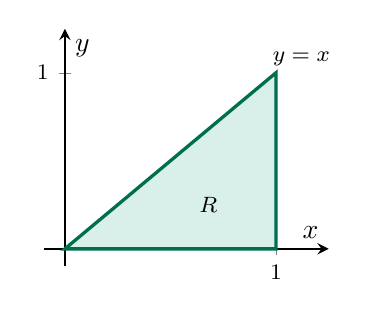
\begin{tikzpicture}
\begin{axis}[width=5.2cm, height=4.6cm, axis lines=middle, xmin=-0.1, xmax=1.25, ymin=-0.1, ymax=1.25,
  xtick={1}, ytick={1}, xlabel={$x$}, ylabel={$y$}, thick, clip=false,
  ticklabel style={font=\footnotesize}]
\fill[gr!15] (axis cs:0,0) -- (axis cs:1,0) -- (axis cs:1,1) -- cycle;
\draw[gr!70!black, very thick] (axis cs:0,0) -- (axis cs:1,0) -- (axis cs:1,1) -- cycle;
\node[font=\footnotesize] at (axis cs:1.12,1.08) {$y=x$};
\node[font=\footnotesize] at (axis cs:0.68,0.25) {$R$};
\end{axis}
\end{tikzpicture}

\footnotesize
$\displaystyle\iint_R xy\,dA = \int_0^1\!\!\int_0^x xy\,dy\,dx = \frac18$
\end{column}
\begin{column}{0.56\textwidth}
\small
volume under $z = f(x,y)$ over $R$:
\[ \iint_R f\,dA = \int_a^b \int_{g(x)}^{h(x)} f(x,y)\,dy\,dx \]

\vspace{0.5em}
\textbf{1.} inner integral first ($y$, with $x$ fixed)\\[4pt]
\textbf{2.} then the outer integral ($x$)
\end{column}
\end{columns}

\vspace{0.6em}
\centering
\cbox{accent!12}{\text{Disks: polar coordinates, } \ dA = r\,dr\,d\theta \quad (\text{don't forget the } r)}
\end{frame}

% ------------------------------------------------------------
\begin{frame}{Monte Carlo integration}
\begin{columns}[T]
\begin{column}{0.40\textwidth}
\centering
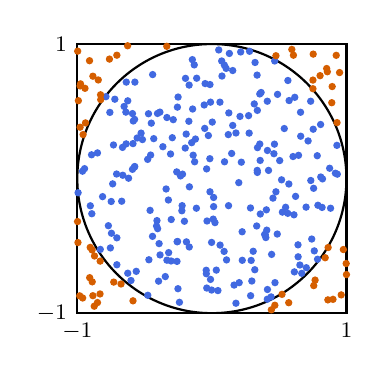
\begin{tikzpicture}
\begin{axis}[width=5.0cm, height=5.0cm, axis equal image, xmin=-1, xmax=1, ymin=-1, ymax=1,
  xtick={-1,1}, ytick={-1,1}, ticklabel style={font=\footnotesize}, thick]
\addplot[only marks, mark=*, mark size=0.9pt, accent] coordinates {(-0.829,-0.526) (0.603,0.164) (-0.812,-0.134) (-0.042,-0.681) (0.469,-0.773) (-0.218,0.033) (-0.139,0.174) (-0.432,0.297) (0.392,-0.415) (-0.403,-0.372) (0.783,0.170) (-0.057,0.547) (-0.252,-0.818) (0.321,0.863) (-0.586,0.260) (-0.404,0.484) (0.444,-0.563) (0.660,0.315) (0.366,0.640) (-0.143,0.517) (0.700,-0.212) (-0.041,-0.707) (0.397,-0.416) (0.742,-0.449) (0.124,-0.201) (0.226,-0.607) (-0.639,0.494) (0.504,0.134) (0.702,-0.662) (0.929,0.247) (0.214,0.941) (0.574,0.580) (-0.892,-0.261) (-0.572,0.717) (-0.746,-0.406) (-0.014,0.699) (-0.573,0.090) (0.412,-0.896) (0.360,-0.263) (0.179,0.339) (0.338,0.046) (0.109,-0.604) (-0.010,-0.749) (-0.039,0.072) (0.548,-0.213) (-0.961,0.055) (-0.590,0.483) (-0.223,-0.239) (0.819,-0.214) (-0.302,-0.304) (-0.038,-0.813) (0.093,0.843) (0.126,0.488) (0.488,0.626) (0.640,-0.492) (-0.036,-0.315) (-0.477,0.143) (-0.364,0.237) (0.165,-0.791) (-0.115,-0.220) (0.413,-0.824) (-0.662,0.025) (-0.191,0.331) (-0.334,-0.606) (-0.706,-0.440) (-0.321,-0.550) (0.073,0.874) (-0.748,-0.170) (0.336,0.769) (0.075,0.762) (-0.894,0.177) (-0.652,0.536) (0.875,0.077) (-0.169,0.695) (-0.526,0.338) (-0.189,-0.470) (0.408,-0.383) (-0.256,0.531) (-0.010,0.568) (0.033,-0.680) (-0.113,0.746) (0.130,0.930) (0.538,0.372) (0.122,0.327) (0.753,0.367) (0.094,0.125) (0.333,-0.352) (0.339,0.230) (0.572,-0.040) (-0.946,0.074) (0.715,0.280) (0.287,-0.218) (-0.287,0.438) (0.788,-0.198) (-0.459,-0.236) (0.319,-0.677) (-0.026,0.320) (0.622,-0.132) (-0.128,0.125) (-0.440,0.773) (-0.576,0.085) (-0.664,0.232) (-0.731,0.250) (0.785,-0.599) (-0.171,0.426) (0.476,-0.098) (0.277,0.338) (-0.294,0.304) (0.155,0.395) (0.023,-0.327) (-0.131,0.845) (-0.625,-0.703) (-0.468,-0.603) (0.200,-0.030) (0.641,-0.581) (0.756,-0.072) (0.616,0.604) (0.822,-0.002) (0.219,0.122) (-0.619,0.003) (-0.346,-0.728) (-0.721,0.590) (0.918,0.040) (-0.233,0.020) (0.659,0.493) (0.735,-0.014) (0.315,0.555) (0.273,0.468) (0.091,-0.541) (0.761,-0.537) (-0.903,-0.202) (-0.340,-0.077) (-0.145,0.884) (-0.334,0.454) (-0.994,-0.105) (0.356,0.257) (0.613,-0.693) (-0.198,0.227) (-0.168,-0.508) (-0.555,0.302) (-0.392,-0.483) (0.461,0.185) (0.808,0.402) (-0.411,-0.352) (-0.754,-0.515) (0.209,0.462) (-0.408,-0.312) (0.518,-0.009) (-0.150,0.267) (-0.167,-0.061) (-0.455,0.175) (-0.590,0.069) (0.809,0.012) (0.654,-0.642) (-0.574,0.440) (-0.396,-0.762) (-0.259,-0.615) (0.734,0.575) (0.337,0.061) (0.051,0.956) (0.045,-0.832) (-0.850,0.191) (0.465,0.256) (0.486,-0.412) (-0.258,-0.469) (-0.255,-0.467) (0.668,-0.704) (-0.584,0.428) (-0.204,-0.317) (-0.562,-0.689) (-0.015,0.148) (-0.307,0.183) (0.356,0.629) (-0.516,0.290) (0.564,-0.258) (-0.014,-0.098) (-0.636,0.717) (-0.323,-0.159) (-0.471,0.482) (0.405,-0.232) (0.013,-0.208) (0.147,0.187) (0.155,0.803) (-0.241,-0.919) (-0.251,0.606) (0.359,0.135) (0.225,-0.395) (-0.625,0.578) (0.003,0.420) (0.179,-0.926) (-0.450,0.412) (-0.303,-0.612) (0.106,0.819) (0.401,-0.438) (0.297,-0.761) (-0.002,-0.474) (0.524,-0.249) (-0.261,0.050) (0.440,-0.879) (0.203,-0.773) (0.338,0.507) (0.882,-0.220) (-0.221,-0.201) (0.412,0.575) (-0.769,-0.350) (0.467,0.874) (-0.196,0.745) (0.010,-0.301) (0.565,0.729) (-0.708,0.034) (-0.706,-0.640) (0.061,-0.494) (0.610,-0.269) (-0.637,0.258) (-0.476,-0.867) (-0.737,-0.039) (0.932,0.033) (0.288,-0.870) (-0.386,0.494) (0.060,0.568) (0.280,0.946) (-0.050,0.706) (0.644,0.173) (0.013,-0.140) (0.292,-0.608) (-0.122,0.294) (-0.385,-0.567) (-0.787,0.609) (0.413,0.209) (-0.053,0.373) (-0.758,0.492) (0.421,0.061) (0.307,-0.540) (-0.002,-0.828) (-0.441,-0.429) (-0.670,-0.168) (0.454,-0.145) (-0.601,-0.757)};
\addplot[only marks, mark=*, mark size=0.9pt, hl] coordinates {(0.476,0.913) (-0.997,0.947) (-0.939,0.414) (0.757,-0.795) (0.842,-0.588) (-0.830,-0.613) (0.930,0.416) (0.894,0.684) (0.864,-0.512) (1.000,-0.713) (-0.982,-0.871) (-0.998,-0.319) (-0.844,0.733) (0.753,0.925) (-0.729,-0.769) (0.442,-0.975) (0.804,0.765) (-0.976,0.704) (0.977,-0.527) (0.853,0.818) (-0.957,0.327) (-0.872,-0.575) (-0.626,0.987) (-0.979,0.382) (-0.761,0.888) (-0.909,0.876) (-0.943,0.671) (-0.904,-0.511) (0.606,0.917) (-0.831,-0.857) (0.521,-0.860) (0.924,0.916) (0.767,-0.754) (-0.826,0.587) (-0.960,-0.887) (0.891,0.564) (0.949,0.788) (-0.884,-0.870) (-0.889,-0.767) (-0.586,-0.908) (0.900,-0.897) (-0.827,0.623) (0.571,-0.922) (-0.908,-0.736) (-0.995,-0.475) (0.862,-0.901) (0.751,0.732) (0.594,0.960) (-0.675,-0.783) (-0.890,-0.530) (0.961,-0.864) (0.998,-0.631) (-0.992,0.579) (-0.850,-0.921) (0.858,0.794) (0.468,-0.941) (-0.979,0.689) (0.751,0.668) (-0.884,0.761) (-0.706,0.917) (-0.874,-0.948) (-0.335,0.983)};
\draw[black, thick] (axis cs:0,0) circle[radius=1];
\end{axis}
\end{tikzpicture}

\footnotesize
$238$ of $300$ inside: \ $\pi \approx 4 \cdot \frac{238}{300} = 3.17$
\end{column}
\begin{column}{0.58\textwidth}
\small
integral $=$ area $\times$ average of $f$
\[ \iint_R f\,dA \;\approx\; |B| \cdot \frac{1}{N}\sum_{i=1}^{N} f(x_i, y_i) \]

\vspace{0.3em}
\textbf{1.} random points in a box $B$ around $R$\\[4pt]
\textbf{2.} $f = 0$ outside $R$\\[4pt]
\textbf{3.} average $\times$ box area

\vspace{0.8em}
\footnotesize
error $\sim 1/\sqrt{N}$, in any dimension
\end{column}
\end{columns}

\vspace{0.6em}
\centering
\cbox{hl!12}{|B| = \text{area of the box you sampled from}}
\end{frame}

\end{document}